\chapter{Technical Framework of Multi-Shot Storyboarding}
\label{ch:multi-shot-storyboards}
\index{storyboards}
\index{multi-shot sequences}

\begin{chapterabstract}
This chapter advances readers from single-shot creation to sophisticated multi-shot sequence construction, establishing technical frameworks for comprehensive visual storytelling. We distinguish between shot thinking (static composition focus) and sequence thinking (temporal narrative flow), demonstrating why the latter is essential for cinematic quality. The chapter presents systematic methodologies for emotional control across sequences, including the emotional arc framework and beat-based rhythm orchestration. We examine visual continuity techniques ensuring coherent transitions between shots, covering match cuts, contrast cuts, and thematic linking strategies. The symbolic language system receives detailed treatment, showing how recurring visual motifs create narrative depth and thematic resonance. Technical frameworks address lighting consistency, color palette progression, and temporal pacing across multi-shot structures. Practical templates provide reusable structures for common narrative patterns including introduction-development-climax-resolution arcs. Through annotated storyboard examples, readers learn to design shot sequences that achieve narrative impact beyond individual frame aesthetics. This chapter transforms creators from image generators into AI directors capable of constructing complex visual narratives through linguistic precision.
\end{chapterabstract}

In AI video creation, single shots function as discrete visual elements, while multi-shot storyboards create comprehensive narrative structures through systematic integration of emotion, lighting, composition, and temporal progression. When creators begin connecting multiple segments systematically, they transition from basic ``image generation'' to advanced ``AI direction.'' This chapter provides technical frameworks for constructing complex visual sequences—covering emotional control, rhythmic orchestration, visual continuity, and symbolic language—ensuring AI-generated content achieves narrative impact beyond aesthetic appeal.\index{narrative impact}

Sora 2 establishes text as the primary tool for shot division and sequence construction\index{text as shot language}. Each Prompt determines both visual presentation and underlying shot logic with embedded emotional beats. Mastering multi-shot storyboard techniques enables creators to \textbf{systematically control temporal narrative} through linguistic precision.

\section{From Shot Thinking to Sequence Thinking: The AI Director's First Step}
\label{sec:shot-to-sequence}
\index{shot thinking}
\index{sequence thinking}

In early short film creation, many newcomers habitually pursue only ``one perfect frame.'' However, true cinematic sense comes from ``continuous rhythm.'' Single-shot thinking is like a photographer's—focused on the present moment; sequence thinking is like a director's—designing holistic flow.

\textbf{Characteristics of Shot Thinking:}

\begin{itemize}
\item Emphasizes static composition and color aesthetics
\item Focuses on character posture, light angle, momentary emotion
\item Similar to photographic works or magazine style
\end{itemize}

\textbf{Characteristics of Sequence Thinking:}

\begin{itemize}
\item Concerns the before-and-after logic and psychological changes of story
\item Uses time to connect visuals, making imagery ``breathe''
\item Each shot is one beat in an emotional movement
\end{itemize}

\begin{Prompt}
Example:

Shot thinking: ``A close-up of a seaside sunset, warm tones.''

Sequence thinking: ``Under the setting sun, she walks alone on the beach—moving slowly forward, pausing, gazing into the distance. Wind sweeps through her hair; she finally turns and walks away.''
\end{Prompt}

\begin{figure}[H]
\centering
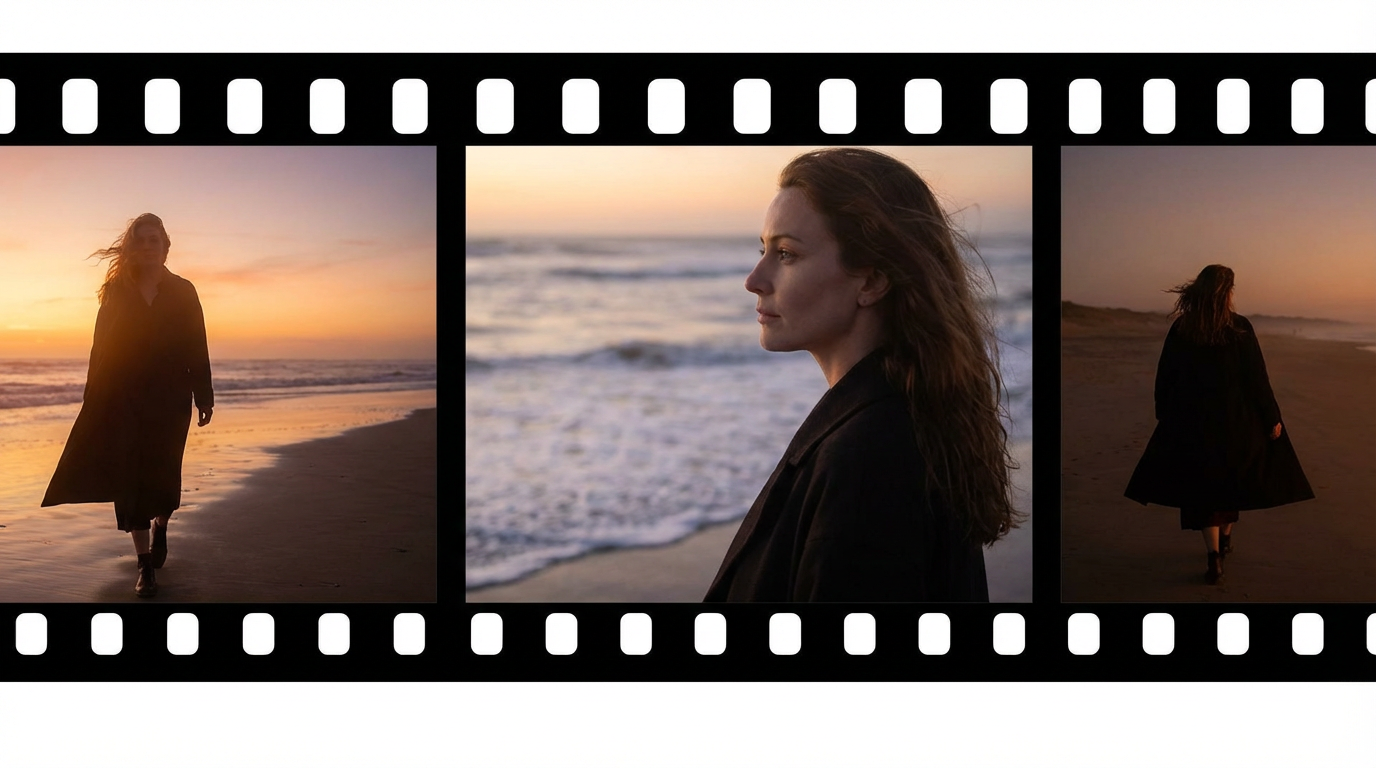
\includegraphics[height=\figheight]{Fig7-1.png}
\caption{Solitary walk on beach—sequence thinking capturing emotional journey \\ \authorcreated}
\label{fig:beach-sequence}
\index{figure!sequence narrative}
\end{figure}

The first example produces static imagery; the second creates narrative progression. AI directors must develop \textbf{narrative association skills}\index{narrative association} to ensure generated content incorporates temporal and emotional dimensions.

\section{Emotional Arc Construction: Systematic Audience Engagement}
\label{sec:emotional-arc}
\index{emotional arc}
\index{psychological journey}

Effective narrative requires emotional foundation. Audience engagement depends on feelings rather than events. AI video creation challenges involve using brief duration to facilitate systematic psychological progression. \textbf{Emotional arc planning}\index{emotional arc} provides the structural framework for this progression \citep{loschky2019scene}.

A simple four-shot emotional flow can form a complete experience:

\textbf{Emotional Flow Example: Hope → Loss → Epiphany → Rebirth}

\begin{enumerate}
\item \textbf{Hope:} Sunlight streams through the window; protagonist packs luggage, lips curved in a smile.

\item \textbf{Loss:} Interview failure; in the glass door's reflection, her face dims.

\item \textbf{Epiphany:} In the rain, she pauses, seeing a slogan in a shop window—``Always Believe in Tomorrow.''

\item \textbf{Rebirth:} Under night lamp, she reopens her laptop, beginning to write the first line of code.
\end{enumerate}

This is the power of AI narrative—in merely 15 seconds, completing an entire psychological journey. Each shot must bear an ``emotional turning point''\index{emotional turning point} to form audience-perceivable rhythm.

You can add emotional keywords to Sora 2 Prompts, for example:

\begin{Prompt}
``a young woman, hopeful, warm sunrise light, gentle camera pan''

``same woman, disappointed, muted colors, slow dolly back shot''
\end{Prompt}

This way AI will automatically generate imagery with greater continuity sense.

\section{Visual Continuity: Making AI's World ``Coherent and Believable''}
\label{sec:visual-continuity}
\index{visual continuity}
\index{coherence in AI}

Sora 2-generated segments are essentially ``multiple independent renders,'' so visual consistency must be artificially constrained through Prompts. Character, lighting, environment, color, camera angle—these are the five major elements of continuity.

\subsection{Character Consistency}
\index{character!consistency}

\begin{itemize}
\item Use identical @ mentions or identical characteristic descriptions
\item Example: @anna, long brown hair, red scarf, gentle expression
\end{itemize}

\subsection{Scene Consistency}
\index{scene!consistency}

\begin{itemize}
\item Clearly specify environmental elements: ``same café window-side table,'' ``same blue wall''
\end{itemize}

\subsection{Lighting Consistency}
\index{lighting!consistency}

\begin{itemize}
\item If shot 1 is in morning light, shot 2 should transition to noon or dusk, not suddenly shift to night
\end{itemize}

\subsection{Color and Atmosphere}
\index{color!consistency}

\begin{itemize}
\item Use keywords to maintain color system, such as ``warm orange light,'' ``teal cinematic tone''
\end{itemize}

\subsection{Camera Angle and Focal Length}
\index{camera angle!consistency}

\begin{itemize}
\item If previous shot is close-up, next shot can use medium or wide angle to create rhythm while preserving spatial logic
\end{itemize}

These five dimensions form the ``physical laws''\index{physical laws of AI narrative} of AI narrative; mastering them makes AI-generated worlds more coherent and realistic.

\section{Transition Techniques: Creating Smooth Shot Sequences}
\label{sec:transition-magic}
\index{transitions!techniques}

Transitions are where AI directors can best demonstrate prowess. Truly smooth AI short films don't rely on editing software but on ``editing within language.''\index{linguistic editing} Research in cognitive science has shown that continuity editing significantly impacts how audiences segment and comprehend narrative events, making smooth transitions crucial for effective storytelling \citep{magliano2011impact}.

\textbf{Common AI Transition Techniques:}

\subsection{Visual Matching (Match Cut)}
\index{match cut}

Two frames ``echo'' through shape, action, or composition.

\begin{Prompt}
``Shot 1: A raindrop falls into water surface.''

``Shot 2: A star falls in the night sky.''
\end{Prompt}

\begin{figure}[H]
\centering
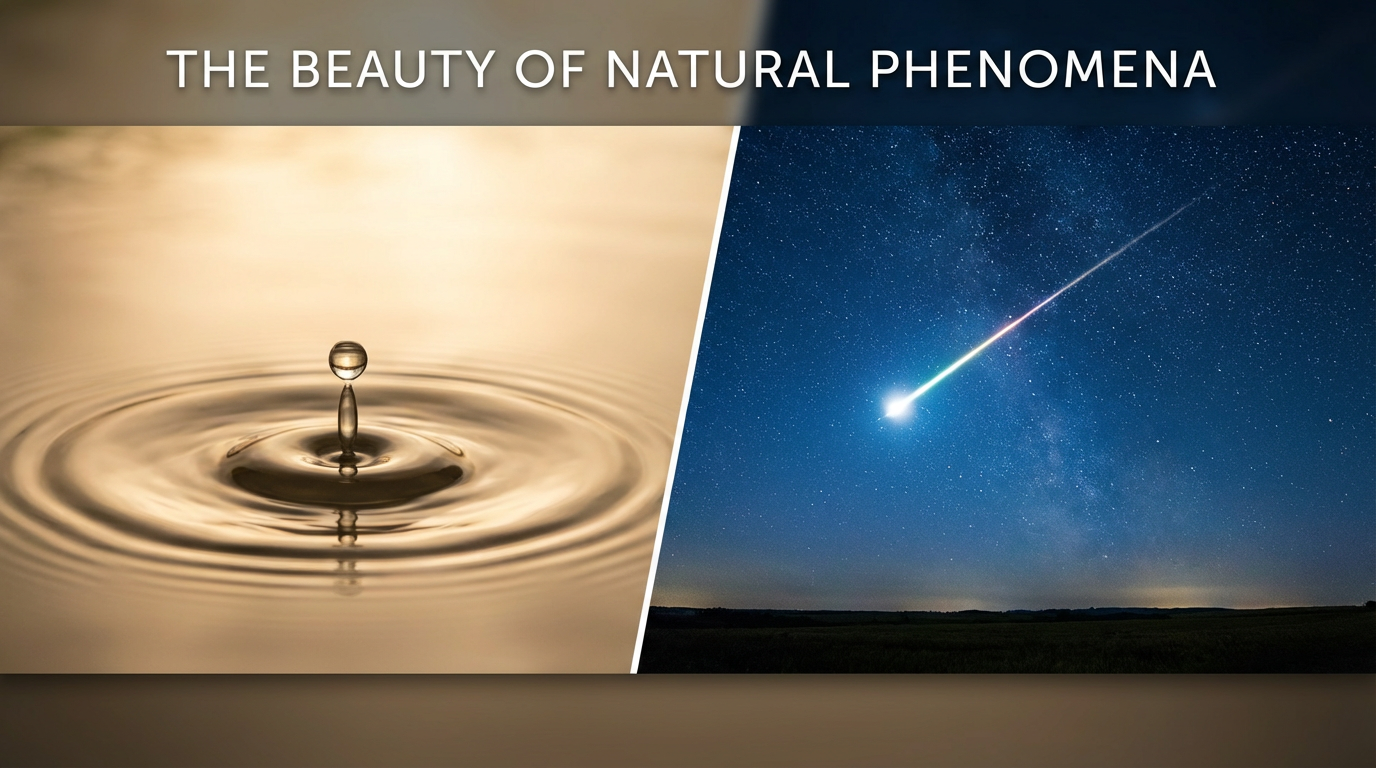
\includegraphics[height=\figheight]{Fig7-2.png}
\caption{Raindrop to falling star—visual match creating poetic connection \\ \authorcreated}
\label{fig:match-cut}
\index{figure!match cut}
\end{figure}

Visually similar yet semantically transformed, forming poetic connection.

\subsection{Motion Transition}
\index{motion transition}

Camera movement direction remains consistent, letting AI continue momentum.

\begin{Prompt}
``Shot 1: Camera follows bird in flight.''

``Shot 2: Camera continues upward; airplane appears skimming clouds.''
\end{Prompt}

\subsection{Color Bridge}
\index{color bridge}

Using same primary hue to transition emotion.

\begin{Prompt}
``Orange sunset → orange-lit café → orange brand LOGO''
\end{Prompt}

\subsection{Emotional Bridge}
\index{emotional bridge}

Forming contrast or continuation emotionally.

\begin{Prompt}
``Child's laughter → years later, adult's relieved smile''
\end{Prompt}

Through this textual ``cinematic language,'' you don't need editing software; you can achieve coherent visual narrative at the Prompt level.

\section{Rhythm: Controlling Audience Breathing and Heartbeat}
\label{sec:rhythm-control}
\index{rhythm!audience control}
\index{breathing frequency}

Rhythm isn't merely fast and slow but the breathing frequency of emotion. AI directors must arrange ``introduction, development, turn, conclusion''\index{four-part structure} like musicians.

\textbf{Rhythm Design Techniques:}

\begin{itemize}
\item \textbf{Rhythm Contrast}\index{rhythm contrast}: Insert a static shot after strong motion shot, like ``running—stopping—deep breath.''

\item \textbf{Shot Length}\index{shot length}: Use different beats to create breathing sense.

\begin{Prompt}
Short shots (2--3 seconds) elevate energy; long shots (6--10 seconds) guide emotional immersion.
\end{Prompt}

\item \textbf{Sound Rhythm}\index{sound rhythm}: Can add ``low ambient hum'' or ``heartbeat sound cue'' in Sora 2, letting AI adjust frame rhythm according to sound dynamics.
\end{itemize}

\textbf{AI Rhythm Script Example:}

\begin{Prompt}
Shot 1: Still room; wind gently sways curtains.

Shot 2: Protagonist rises and rushes out door; camera shakes.

Shot 3: Close-up, breathing rapid, background blurred.

Shot 4: Outside door, sunlight piercing; he stops, takes deep breath.
\end{Prompt}

\begin{figure}[H]
\centering
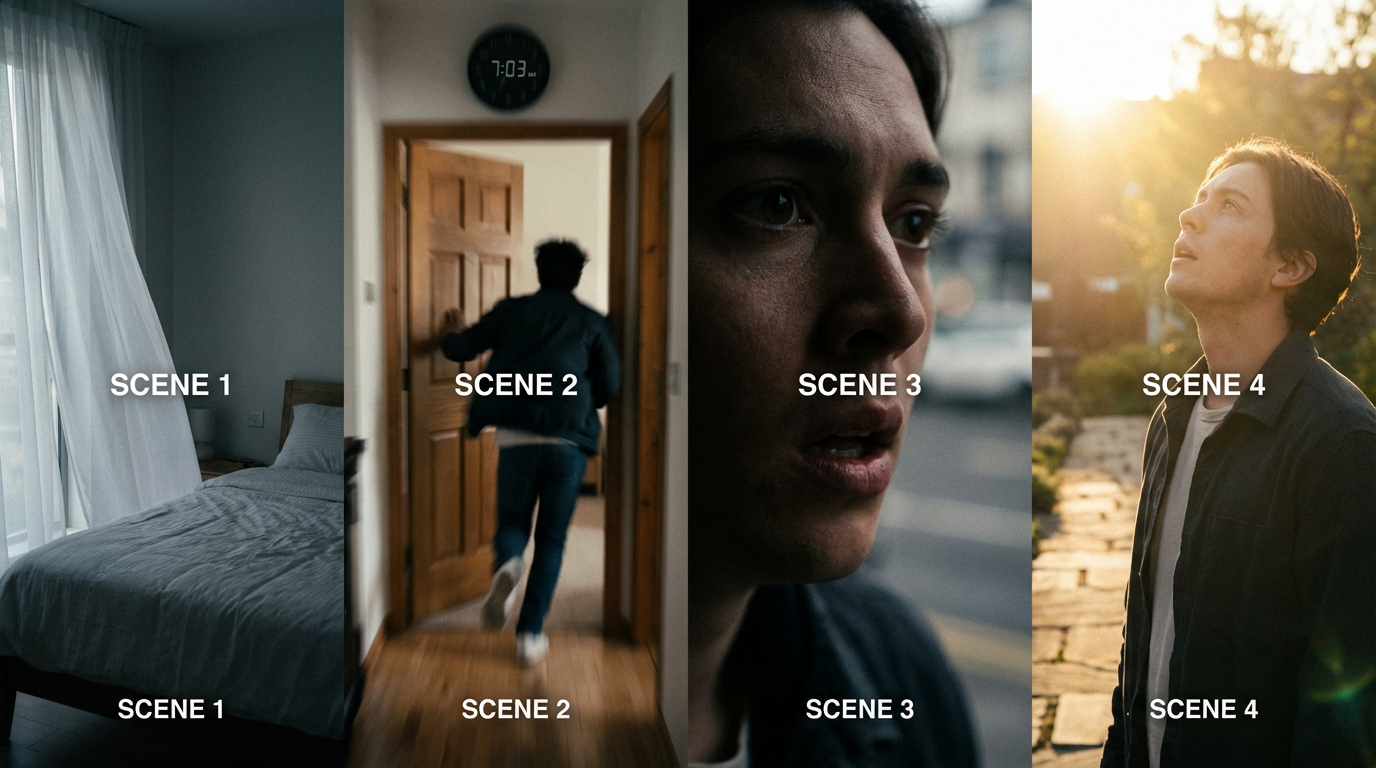
\includegraphics[height=\figheight]{Fig7-3.png}
\caption{From stillness to motion to stillness—rhythmic tension and release \\ \authorcreated}
\label{fig:rhythm-tension}
\index{figure!rhythmic design}
\end{figure}

This ``tension and release''\index{tension and release} design creates deeper resonance emotionally.

\section{Iterative Creation Method: Polishing Repeatedly Like a Director}
\label{sec:iterative-creation}
\index{iterative creation}
\index{refinement process}

AI video isn't a one-time finished work but a process of multi-round debugging. Can execute according to following steps:

\begin{enumerate}
\item \textbf{First Round (Sketch Stage):} Write only main scenes and characters.

\item \textbf{Second Round (Connection Stage):} Add continuity descriptions and transition cues.

\item \textbf{Third Round (Polish Stage):} Optimize light, action, rhythm vocabulary.

\item \textbf{Fourth Round (Music and Atmosphere):} Add environmental sound, color palette, psychological hints.
\end{enumerate}

\begin{Prompt}
Example:

\begin{itemize}
\item Round 1: ``Woman sits in café.''
\item Round 2: ``Woman sits in café, red scarf, rain outside.''
\item Round 3: ``Woman in red scarf gazes at door; rain light reflects in her eyes.''
\end{itemize}
\end{Prompt}

AI's power lies in allowing you to become a director with ``infinite retakes.''\index{infinite retakes} Each revision can make emotion more precise.

\section{Storyboard Templates: Customizing Structures for Different Types}
\label{sec:storyboard-templates}
\index{storyboard templates}

\subsection{Three-Act Nine-Shot Structure}
\index{three-act structure}

\begin{itemize}
\item Beginning: Character, background, motivation
\item Conflict: Obstacle, misunderstanding, challenge
\item Resolution: Choice, transformation, calm
\end{itemize}

\subsection{Five-Shot Emotional Journey}
\index{emotional journey}

\begin{itemize}
\item Calm → Trigger → Peak → Collapse → Rebirth
\end{itemize}

\subsection{Eight-Shot Product Ad Structure}
\index{product advertising!structure}

\begin{enumerate}
\item User pain point
\item Product appearance
\item Feature demonstration
\item Usage experience
\item Life transformation
\item Brand emotional resonance
\item Logo close-up
\item Slogan fade-out
\end{enumerate}

\section{Advanced Techniques: Temporal and Spatial Control in AI Narrative}
\label{sec:advanced-techniques}
\index{advanced techniques}

\begin{itemize}
\item \textbf{Parallel Editing}\index{parallel editing}: Switching back and forth between two scenes, creating contrast and tension.

\item \textbf{Time Jumps}\index{time jumps}: Showing growth, seasons, life's passage.

\item \textbf{Perspective Shifts}\index{perspective shifts}: Telling the same event from different character or object viewpoints.

\item \textbf{Symbolic Recurrence}\index{symbolic recurrence}: Certain objects repeatedly appear (like window light, raindrops, mirrors), becoming thematic threads.
\end{itemize}

\begin{Prompt}
Example: ``Girl first looks in mirror → years later gazes again → reflection in mirror smiles.''
\end{Prompt}

This ``symbolic recurrence'' is the most poetic technique in AI visual narrative.

\begin{figure}[H]
\centering
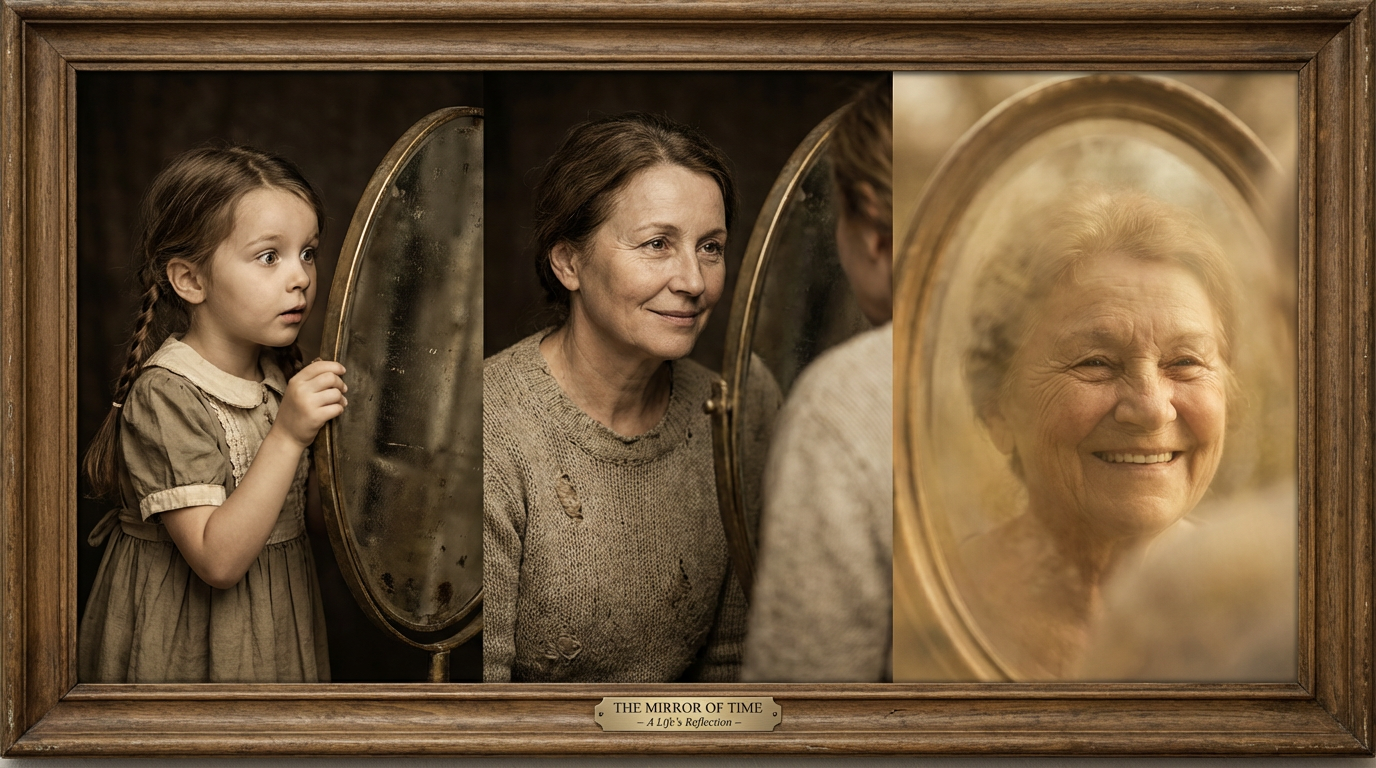
\includegraphics[height=\figheight]{Fig7-4.png}
\caption{Mirror motif across time—symbolic recurrence as narrative thread \\ \authorcreated}
\label{fig:mirror-recurrence}
\index{figure!symbolic recurrence}
\end{figure}

\section{Common Issues and Correction Strategies}
\label{sec:common-issues}
\index{troubleshooting}

\begin{table}[H]
\centering
\caption{Common storyboard issues and solutions \\ \authorillustration}
\label{tab:storyboard-issues}
\index{table!troubleshooting}
\begin{tabular}{p{3cm}p{4cm}p{6cm}}
\hline
\textbf{Issue} & \textbf{Symptom} & \textbf{Adjustment Strategy} \\
\hline
Visual inconsistency & Character or background sudden change & Lock character description + repeat location elements \\
Lighting inconsistency & Before-after light conflict & Specify time period and weather conditions \\
Rhythm fracture & Shot length disordered & Unify each shot's time interval \\
Emotional defocus & Audience feeling vague & Add specific emotion words to Prompts (sad/relieved/calm) \\
Style drift & Color tone or composition style changes & Add style-locking words globally, such as ``cinematic, shallow depth of field'' \\
\hline
\end{tabular}
\end{table}

\section{Testing and Feedback: Breathing Life into Your Work}
\label{sec:testing-feedback}
\index{feedback}
\index{testing}

After completing initial version, should examine like an audience:

\begin{itemize}
\item Does \textbf{emotional curve} progress naturally?
\item Is \textbf{visual consistency} coherent?
\item Do \textbf{rhythm and sound effects} coordinate?
\item Is the \textbf{core memorable moment} strong enough?
\end{itemize}

\begin{Prompt}
Tip: Invite third parties to watch; record moments of their emotional fluctuation—that's evidence of effective rhythm.
\end{Prompt}

\section{From Sequence to Short Film: Mastering ``The Art of Combination''}
\label{sec:sequence-to-film}
\index{combination art}

A sequence is only the starting point; a true AI short film is the assembly of multiple sequences. After mastering multi-shot design, you can:

\begin{itemize}
\item Combine 3 independent emotional arcs into 1-minute narrative
\item Use visual symbols to thread through multiple chapters
\item Form a ``worldview''\index{worldview building} in Sora 2 through consistent characters, tones, objects
\end{itemize}

As the Kuleshov experiment\index{Kuleshov effect} demonstrated: emotion doesn't come from shots but from connections between shots. This principle aligns with modern theories of scene perception and event comprehension, which explain how viewers construct narrative understanding through the cognitive processing of visual sequences \citep{loschky2019scene}.

Master connections, and you master cinema's language.

\section*{Practical Exercises}
\index{storyboard exercises}

\begin{quote}
\textit{\textbf{Timeless Principle:} Even as interfaces evolve and platforms update, the underlying visual logic---light, composition, rhythm, and emotional resonance---remains eternal. Master these fundamentals, and you will adapt effortlessly to any future tool.}
\end{quote}

\subsection*{Exercise 1: Three-Beat Emotional Arc}
\textbf{Objective:} Master basic emotional progression in multi-shot sequences

\textbf{Scenario:} A person receiving unexpected news

\textbf{Instructions:}
\begin{enumerate}
\item \textbf{Beat 1 (Setup):} Create a Prompt showing the character in their normal state
   \begin{itemize}
   \item Example: "Young woman reading peacefully in café, soft afternoon light, relaxed posture, gentle background ambiance"
   \end{itemize}
\item \textbf{Beat 2 (Disruption):} Show the moment of change
   \begin{itemize}
   \item Example: "Same woman looking at phone screen, expression shifting from calm to surprise, camera slowly pushing in, lighting subtly dimming"
   \end{itemize}
\item \textbf{Beat 3 (Resolution):} Reveal the emotional outcome
   \begin{itemize}
   \item Example: "Close-up of woman's face breaking into joyful smile, tears of happiness, warm light returning, camera pulling back to show her celebration"
   \end{itemize}
\item Generate all three shots and evaluate the emotional flow
\item Experiment with different news types (good/bad/mysterious) and adjust accordingly
\end{enumerate}

\subsection*{Exercise 2: Visual Continuity Challenge}
\textbf{Objective:} Maintain consistent visual elements across multiple shots

\textbf{Base Elements to Maintain:}
\begin{itemize}
\item Character: Same person in consistent clothing
\item Environment: Kitchen setting with specific props
\item Lighting: Golden hour sunlight through window
\item Color Palette: Warm earth tones with blue accents
\end{itemize}

\textbf{Shot Sequence to Create:}
\begin{enumerate}
\item Wide shot establishing the kitchen scene
\item Medium shot of character cooking
\item Close-up of hands preparing ingredients
\item Extreme close-up of food sizzling in pan
\item Return to medium shot showing character's satisfaction
\end{enumerate}

\textbf{Evaluation Criteria:}
\begin{itemize}
\item Does lighting remain consistent across all shots?
\item Are character details (clothing, appearance) maintained?
\item Do props and environmental elements stay in logical positions?
\item Is the color palette harmonious throughout?
\end{itemize}

\subsection*{Exercise 3: Transition Technique Practice}
\textbf{Objective:} Master different types of shot transitions

\textbf{Transition Types to Practice:}
\begin{enumerate}
\item \textbf{Match Cut:} "Hand reaching for door handle" → "Hand reaching for car door handle"
\item \textbf{Graphic Match:} "Full moon in night sky" → "White plate on dark table"
\item \textbf{Motion Match:} "Bird flying left to right" → "Airplane flying left to right"
\item \textbf{Eye-line Match:} "Person looking up with wonder" → "Fireworks exploding in sky"
\item \textbf{Sound Bridge:} "Person speaking" → "Same voice continuing over different location"
\end{enumerate}

\section*{Storyboard Templates}
\index{storyboard templates}

\subsection*{Template 1: Character Journey Arc}
\textbf{Structure:} Establishment → Challenge → Transformation → Resolution

\textbf{Shot Breakdown:}
\begin{enumerate}
\item \textbf{Establishing Shot:} "[Character] in [familiar environment], [normal activity], [baseline emotional state], [consistent lighting/color scheme]"
\item \textbf{Inciting Incident:} "[Character] encounters [challenge/change], [camera movement toward character], [lighting shift], [emotional transition begins]"
\item \textbf{Struggle/Process:} "[Character] [action showing effort/change], [dynamic camera work], [evolving lighting], [internal conflict visible]"
\item \textbf{Resolution:} "[Character] [final state/achievement], [camera position showing outcome], [lighting reflecting resolution], [emotional payoff clear]"
\end{enumerate}

\subsection*{Template 2: Product/Brand Showcase}
\textbf{Structure:} Context → Product Introduction → Demonstration → Lifestyle Integration

\textbf{Shot Breakdown:}
\begin{enumerate}
\item \textbf{Lifestyle Context:} "[Target audience] in [relevant situation], [problem/need apparent], [natural lighting], [relatable environment]"
\item \textbf{Product Reveal:} "[Product] [elegant introduction], [hero lighting], [clean background], [focus on key features]"
\item \textbf{Demonstration:} "[Product in use], [dynamic angles showing function], [benefit clearly visible], [user satisfaction evident]"
\item \textbf{Integration:} "[Product seamlessly part of lifestyle], [wide shot showing harmony], [aspirational lighting], [emotional satisfaction]"
\end{enumerate}

\subsection*{Template 3: Atmospheric Mood Piece}
\textbf{Structure:} Environment → Details → Human Element → Synthesis

\textbf{Shot Breakdown:}
\begin{enumerate}
\item \textbf{Wide Establishing:} "[Location] at [specific time], [weather/atmospheric conditions], [overall mood], [color temperature]"
\item \textbf{Environmental Details:} "[Specific elements] that [convey mood], [macro/close-up shots], [texture and movement], [sensory details]"
\item \textbf{Human Presence:} "[Character] [interacting with environment], [scale showing relationship], [emotional resonance], [natural integration]"
\item \textbf{Synthesis:} "[Wide shot] showing [harmony between human and environment], [emotional culmination], [thematic resolution]"
\end{enumerate}

\section*{Storyboard Quality Checklist}
\index{storyboard checklist}

\subsection*{Pre-Production Planning}
Before creating your storyboard:

\begin{itemize}
\item[$\square$] \textbf{Emotional Arc Mapped}: Have you identified 3-5 key emotional beats?
\item[$\square$] \textbf{Visual Consistency Plan}: Are lighting, color, and style guidelines established?
\item[$\square$] \textbf{Character Continuity}: Are character details (clothing, appearance, props) documented?
\item[$\square$] \textbf{Transition Strategy}: Have you planned how shots will connect?
\item[$\square$] \textbf{Pacing Structure}: Are shot durations planned for desired rhythm?
\item[$\square$] \textbf{Technical Requirements}: Are resolution, aspect ratio, and format specifications clear?
\end{itemize}

\subsection*{Shot-by-Shot Evaluation}
For each individual shot:

\begin{itemize}
\item[$\square$] \textbf{Narrative Purpose}: Does this shot advance the story or emotion?
\item[$\square$] \textbf{Visual Clarity}: Is the composition clear and readable?
\item[$\square$] \textbf{Emotional Contribution}: Does the shot support the intended mood?
\item[$\square$] \textbf{Technical Quality}: Are camera movement and lighting appropriate?
\item[$\square$] \textbf{Continuity Compliance}: Does it match established visual rules?
\item[$\square$] \textbf{Transition Readiness}: Will it connect smoothly to adjacent shots?
\end{itemize}

\subsection*{Sequence-Level Assessment}
For the complete storyboard:

\begin{itemize}
\item[$\square$] \textbf{Emotional Flow}: Does the sequence create a satisfying emotional journey?
\item[$\square$] \textbf{Visual Coherence}: Do all shots feel like part of the same world?
\item[$\square$] \textbf{Pacing Effectiveness}: Does the rhythm support the narrative goals?
\item[$\square$] \textbf{Narrative Clarity}: Is the story/message clear without explanation?
\item[$\square$] \textbf{Technical Consistency}: Are all shots technically compatible for editing?
\item[$\square$] \textbf{Audience Engagement}: Will viewers remain emotionally invested throughout?
\end{itemize}

\subsection*{Revision and Refinement}
When revising your storyboard:

\begin{enumerate}
\item \textbf{Identify Weak Points}: Which shots feel disconnected or unclear?
\item \textbf{Test Emotional Beats}: Do the highs and lows occur at the right moments?
\item \textbf{Verify Transitions}: Are all shot connections smooth and logical?
\item \textbf{Check Pacing}: Are any sections too rushed or too slow?
\item \textbf{Validate Consistency}: Do visual elements remain coherent throughout?
\item \textbf{Seek External Feedback}: How do others respond to the emotional flow?
\end{enumerate}

\section*{Chapter Summary}

Key actionable insights for multi-shot storyboarding:

\begin{itemize}
\item \textbf{Emotional Arc Design}: Map 3-5 emotional beats before writing Prompts to ensure narrative progression
\item \textbf{Visual Continuity}: Maintain consistent lighting, color palette, and character positioning across shots
\item \textbf{Transition Planning}: Use specific transition words (``cut to,'' ``fade in,'' ``match cut'') in Prompts for smooth flow
\item \textbf{Rhythm Control}: Vary shot lengths (2-4 seconds for action, 4-6 seconds for emotion) to create dynamic pacing
\item \textbf{Third-Party Testing}: Show sequences to others and note their emotional responses to validate effectiveness
\end{itemize}

\section*{Summary}

This chapter teaches not only technique but the transformation of narrative thinking. AI directors must learn to make language become shots, shots become emotion, emotion become story. In the next chapter, we'll conduct hands-on practice based on a real image—how to generate complete advertising-grade video through Sora 2, from conception to composition to copywriting presentation, creating your first ``AI director short film.''
